\section{Long-Tail Issue}
In previous research, three main groups of techniques have been employed to deal with the long-tail issue: Re-weighting, Re-sampling, and Few-Shot Learning.

\subsection{Re-weighting}
Re-weighting is a technique used to apply varying weights of penalty to specific groups of classes or samples. This is typically achieved by modifying the loss function. The most vanilla re-weighting scheme involves applying the inverse class frequency to the loss. In this manner, more frequent classes receive a lower weight of loss, enabling the model to put more emphasis on the tail classes \parencite{khan2017cost, mostajabi2015feedforward}.

However, it has been proved that as the number of samples increases, the marginal benefit of model performance diminishes. As a result, directly applying the inverse class frequency to the loss function may excessively reduce the weight of losses for the frequent classes. Class Balanced Loss (CB Loss) has been proposed to resolve this issue. As illustrated in Figure \ref{fig:concetpcbloss}, CB Loss calculates the effective number of samples to balance the inverse class frequency, yielding a more reasonable weight for the loss \parencite{cui2019class}.

\begin{figure}[ht]
    \centering
    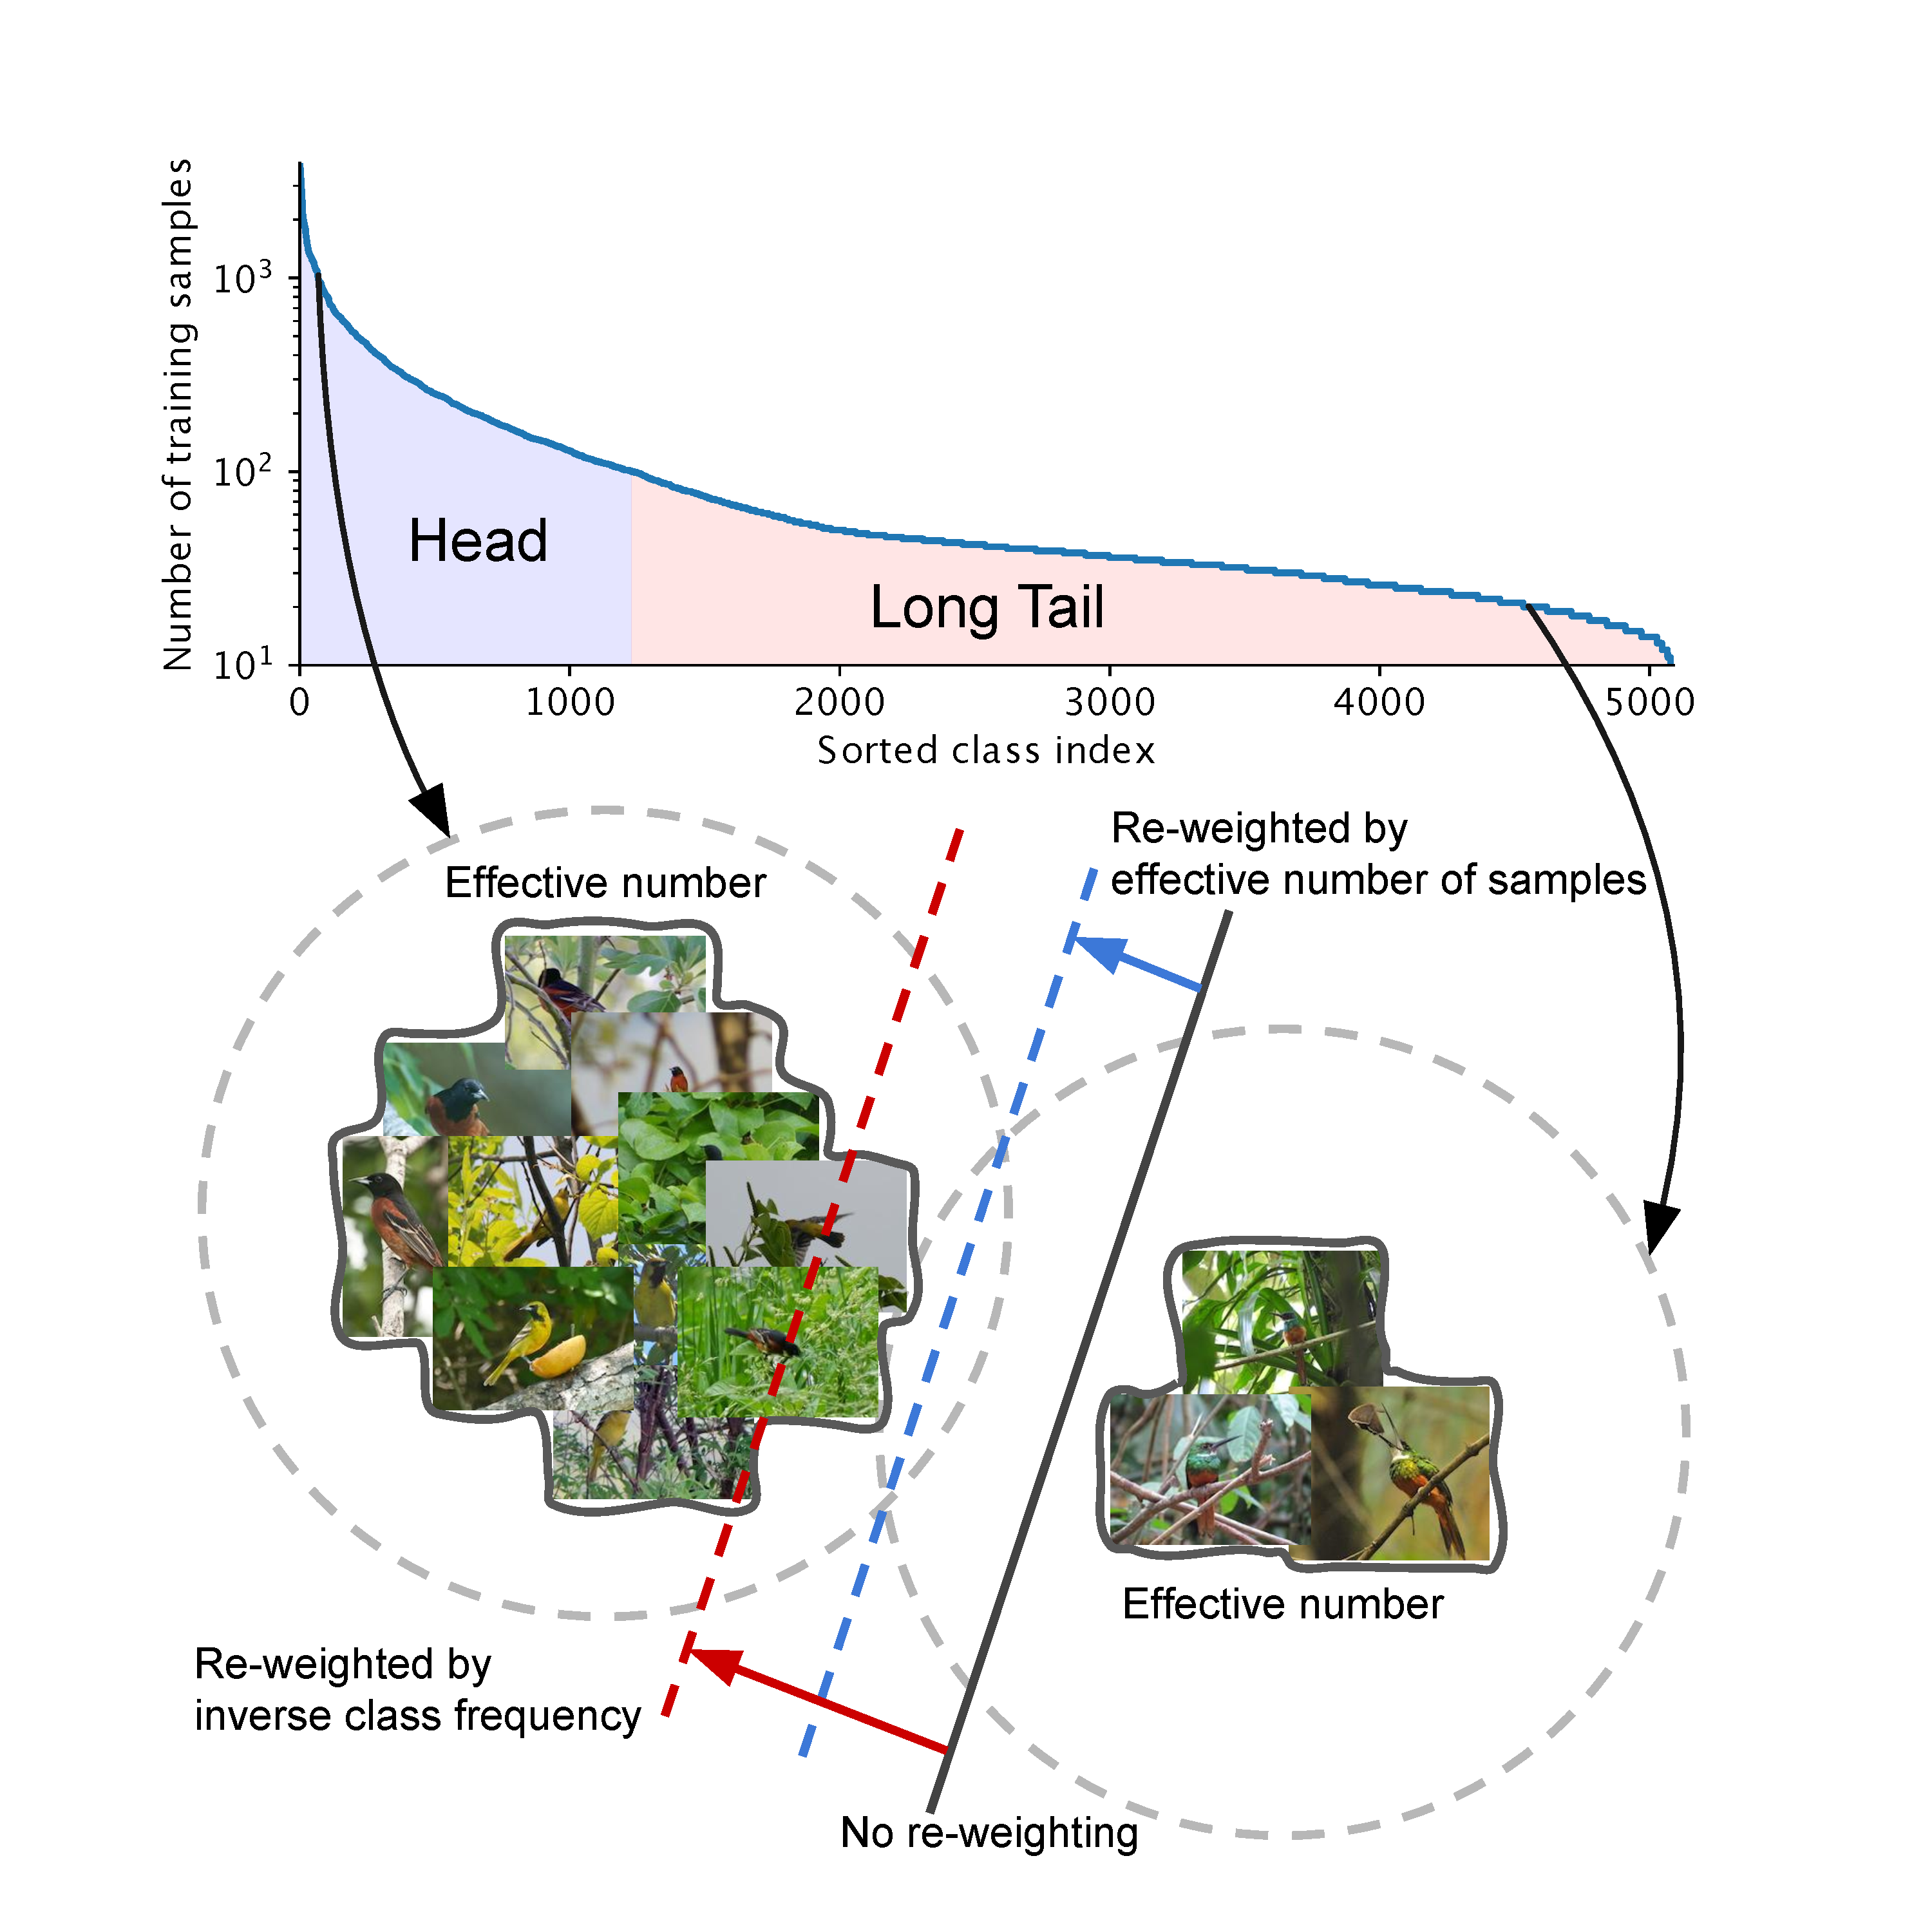
\includegraphics[width=0.5\textwidth]{assets/charts_rw/CBLoss}
    \caption[CB Loss illustration]{This chart illustrates the concept of CB Loss. The effective number of samples is calculated for re-weighting. Source: \parencite{cui2019class}}
    \label{fig:concetpcbloss}
\end{figure}

In contrast to frequency-based re-weighting, Focal Loss focuses on the level of learning difficulties. It scales the penalty to automatically down-weight the contribution of easy examples, which enforces the model to focus on the hard examples \parencite{lin2017focal}.

Label-Distribution-Aware Margin (LDAM) Loss, inspired by the hinge loss in Support Vector Machine, ensures that the model establishes a closer decision boundary while classifying frequent classes, as illustrated in Figure \ref{fig:concetpldam}, to provide room for the less frequent class with more uncertainty. This implies that the model is required to produce higher confidence probabilities to achieve a better performance \parencite{cao2019learning}.

\begin{figure}[ht]
    \centering
    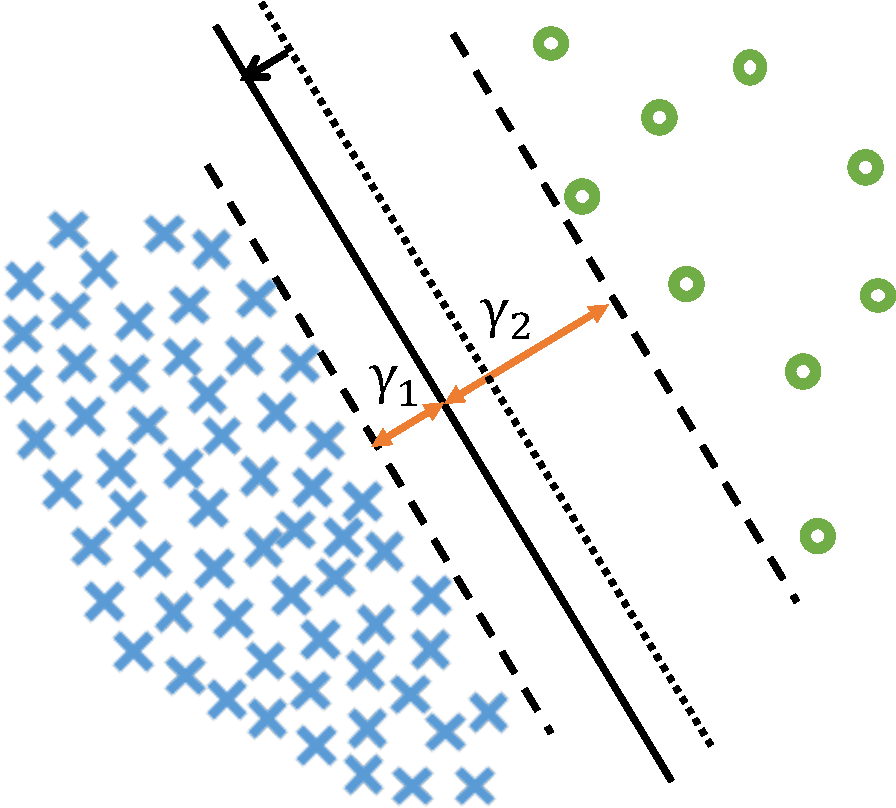
\includegraphics[width=0.5\textwidth]{assets/charts_rw/LDAM}
    \caption[LDAM illustration]{This chart illustrates the concept of LDAM. The decision boundary is adjusted toward the frequent class to provide room for the less frequent class with more uncertainty. Source: \parencite{cao2019learning}}
    \label{fig:concetpldam}
\end{figure}

In the context of videos, re-weighting may not be the best strategy to overcome the long-tail issue. Considering the varying amounts of information in a single video, adjusting the weights to tail classes is likely to introduce noise into the training process \parencite{zhang2021videolt}. 

\subsection{Re-sampling}
Re-sampling refers to the intuitive use of sampling algorithms to balance the number of samples for each class. Several early research studies have applied this technique to enhance the model performance \parencite{shen2016relay, 5128907, mahajan2018exploring}.

Previous research has also found that data imbalance itself does not affect the performance of representation learning. Although re-sampling has led to better performance in classification results, it actually benefits classifier learning while harming representation learning. Consequently, subsequent research has focused more on re-sampling techniques used in classifier training \parencite{zhou2020bbn, kang2019decoupling}.

Compared to the previous method that focused on re-sampling algorithms, subsequent research has attempted to reconstruct more samples. For instance, VideoLT concatenates frames from different videos to generate additional tail samples \parencite{zhang2021videolt}. Similarly, reconstruction of samples in the embedding space has also been explored by researchers \parencite{liu2022long, perrett2023use}. For example, Long-Tail Mixed Reconstruction \parencite{perrett2023use}, as illustrated in Figure \ref{fig:augembedding}, decomposes the entire model into image encoder and classifier and reconstructs samples using the embeddings generated by the image encoder.

\begin{figure}[ht]
    \centering
    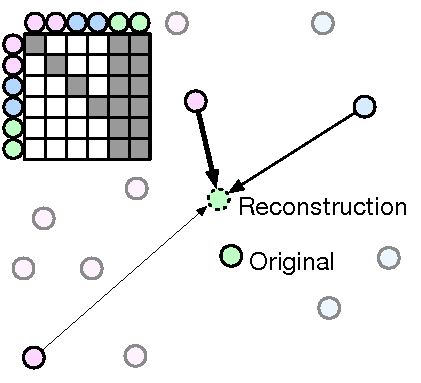
\includegraphics[width=0.5\textwidth]{assets/charts_rw/AugEmbedding}
    \caption[Illustration of Reconstruction of Samples in the Embedding Space]{This chart illustrates the concept of reconstructing samples in the embedding space. Tail samples in green colour are reconstructed by other samples in the batch using the weighted sum method. Samples on the row axis in the matrix on the top-left of the figure denote the features to be reconstructed, while sample on the column axis implies the features being used for the reconstruction. The cells in grey colour are masked out for the weighted sum calculation. Source: \parencite{perrett2023use}}
    \label{fig:augembedding}
\end{figure}

These re-sampling techniques certainly mitigate poor performance in the tail classes. Nevertheless, they do not guarantee the production of samples with the same variety and correctness as the collected data.

\subsection{Few-Shot Learning}
More recent research is concentrating on learning techniques that require fewer training data to achieve acceptable performance.

Model-Agnostic Meta-Learning (Moco) \parencite{finn2017model} introduced the concept of learning to initialise better parameters for training. This has led to a series of studies on meta-learning. Apart from initialisation \parencite{nichol2018first, 2018Reptile}, a large amount of research has emerged, applying meta-learning to various aspects, such as searching for optimization techniques \parencite{andrychowicz2016learning}, data augmentation strategies \parencite{li2020dada, galashov2022data, cubuk2018autoaugment}, and even re-weighting strategies \parencite{shu2019meta}. For instance, Figure \ref{fig:concetpdada} illustrates the concept of Differential Automation Data Augmentation (DADA) \parencite{li2020dada}, which explores a differentiable approach to image augmentation for meta-learning.

\begin{figure}[ht]
    \centering
    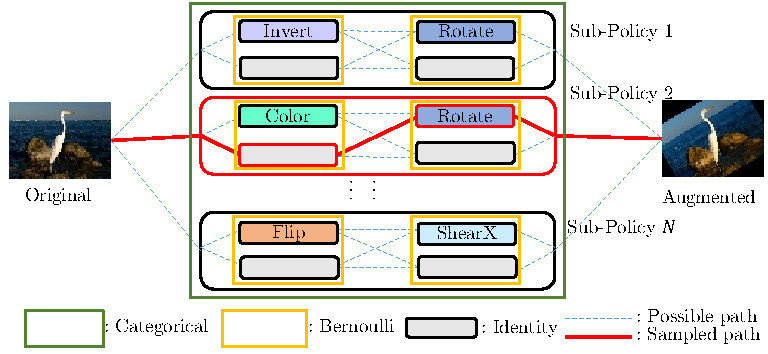
\includegraphics[width=0.8\textwidth]{assets/charts_rw/DADA}
    \caption[Illustration of Differential Automation Data Augmentation]{This figure illustrates the concept of Differential Automation Data Augmentation. Source: \parencite{li2020dada}}
    \label{fig:concetpdada}
\end{figure}

With the ability to learn from the small size of data, few-shot learning techniques can also mitigate the long-tail issue. MetaModelNet, for example, regresses the parameters from models trained with less data to the parameters from models trained with more data \parencite{NIPS2017_147ebe63}. Besides, some studies have shown that augmentation or memory retrieval in the embedding space are effective ways to handle tail classes \parencite{liu2019large, Zhu_2020_CVPR, li2021metasaug, Fu_2022_ACCV}.

These approaches primarily either concentrate on few-shot learning or generalise the representation learned from the head classes to the tail classes. In contrast with these methods, Contrastive Vision-Language Pre-training (CLIP) \parencite{radford2021learning} embeds both images and sentences into a unified semantic space, as illustrated in Figure \ref{fig:clipstructure}. This empowers the model to effectively leverage human intelligence to understand visual data as well as balance the distribution of learning targets \parencite{ma2022x}. 

\begin{figure}[ht]
    \centering
    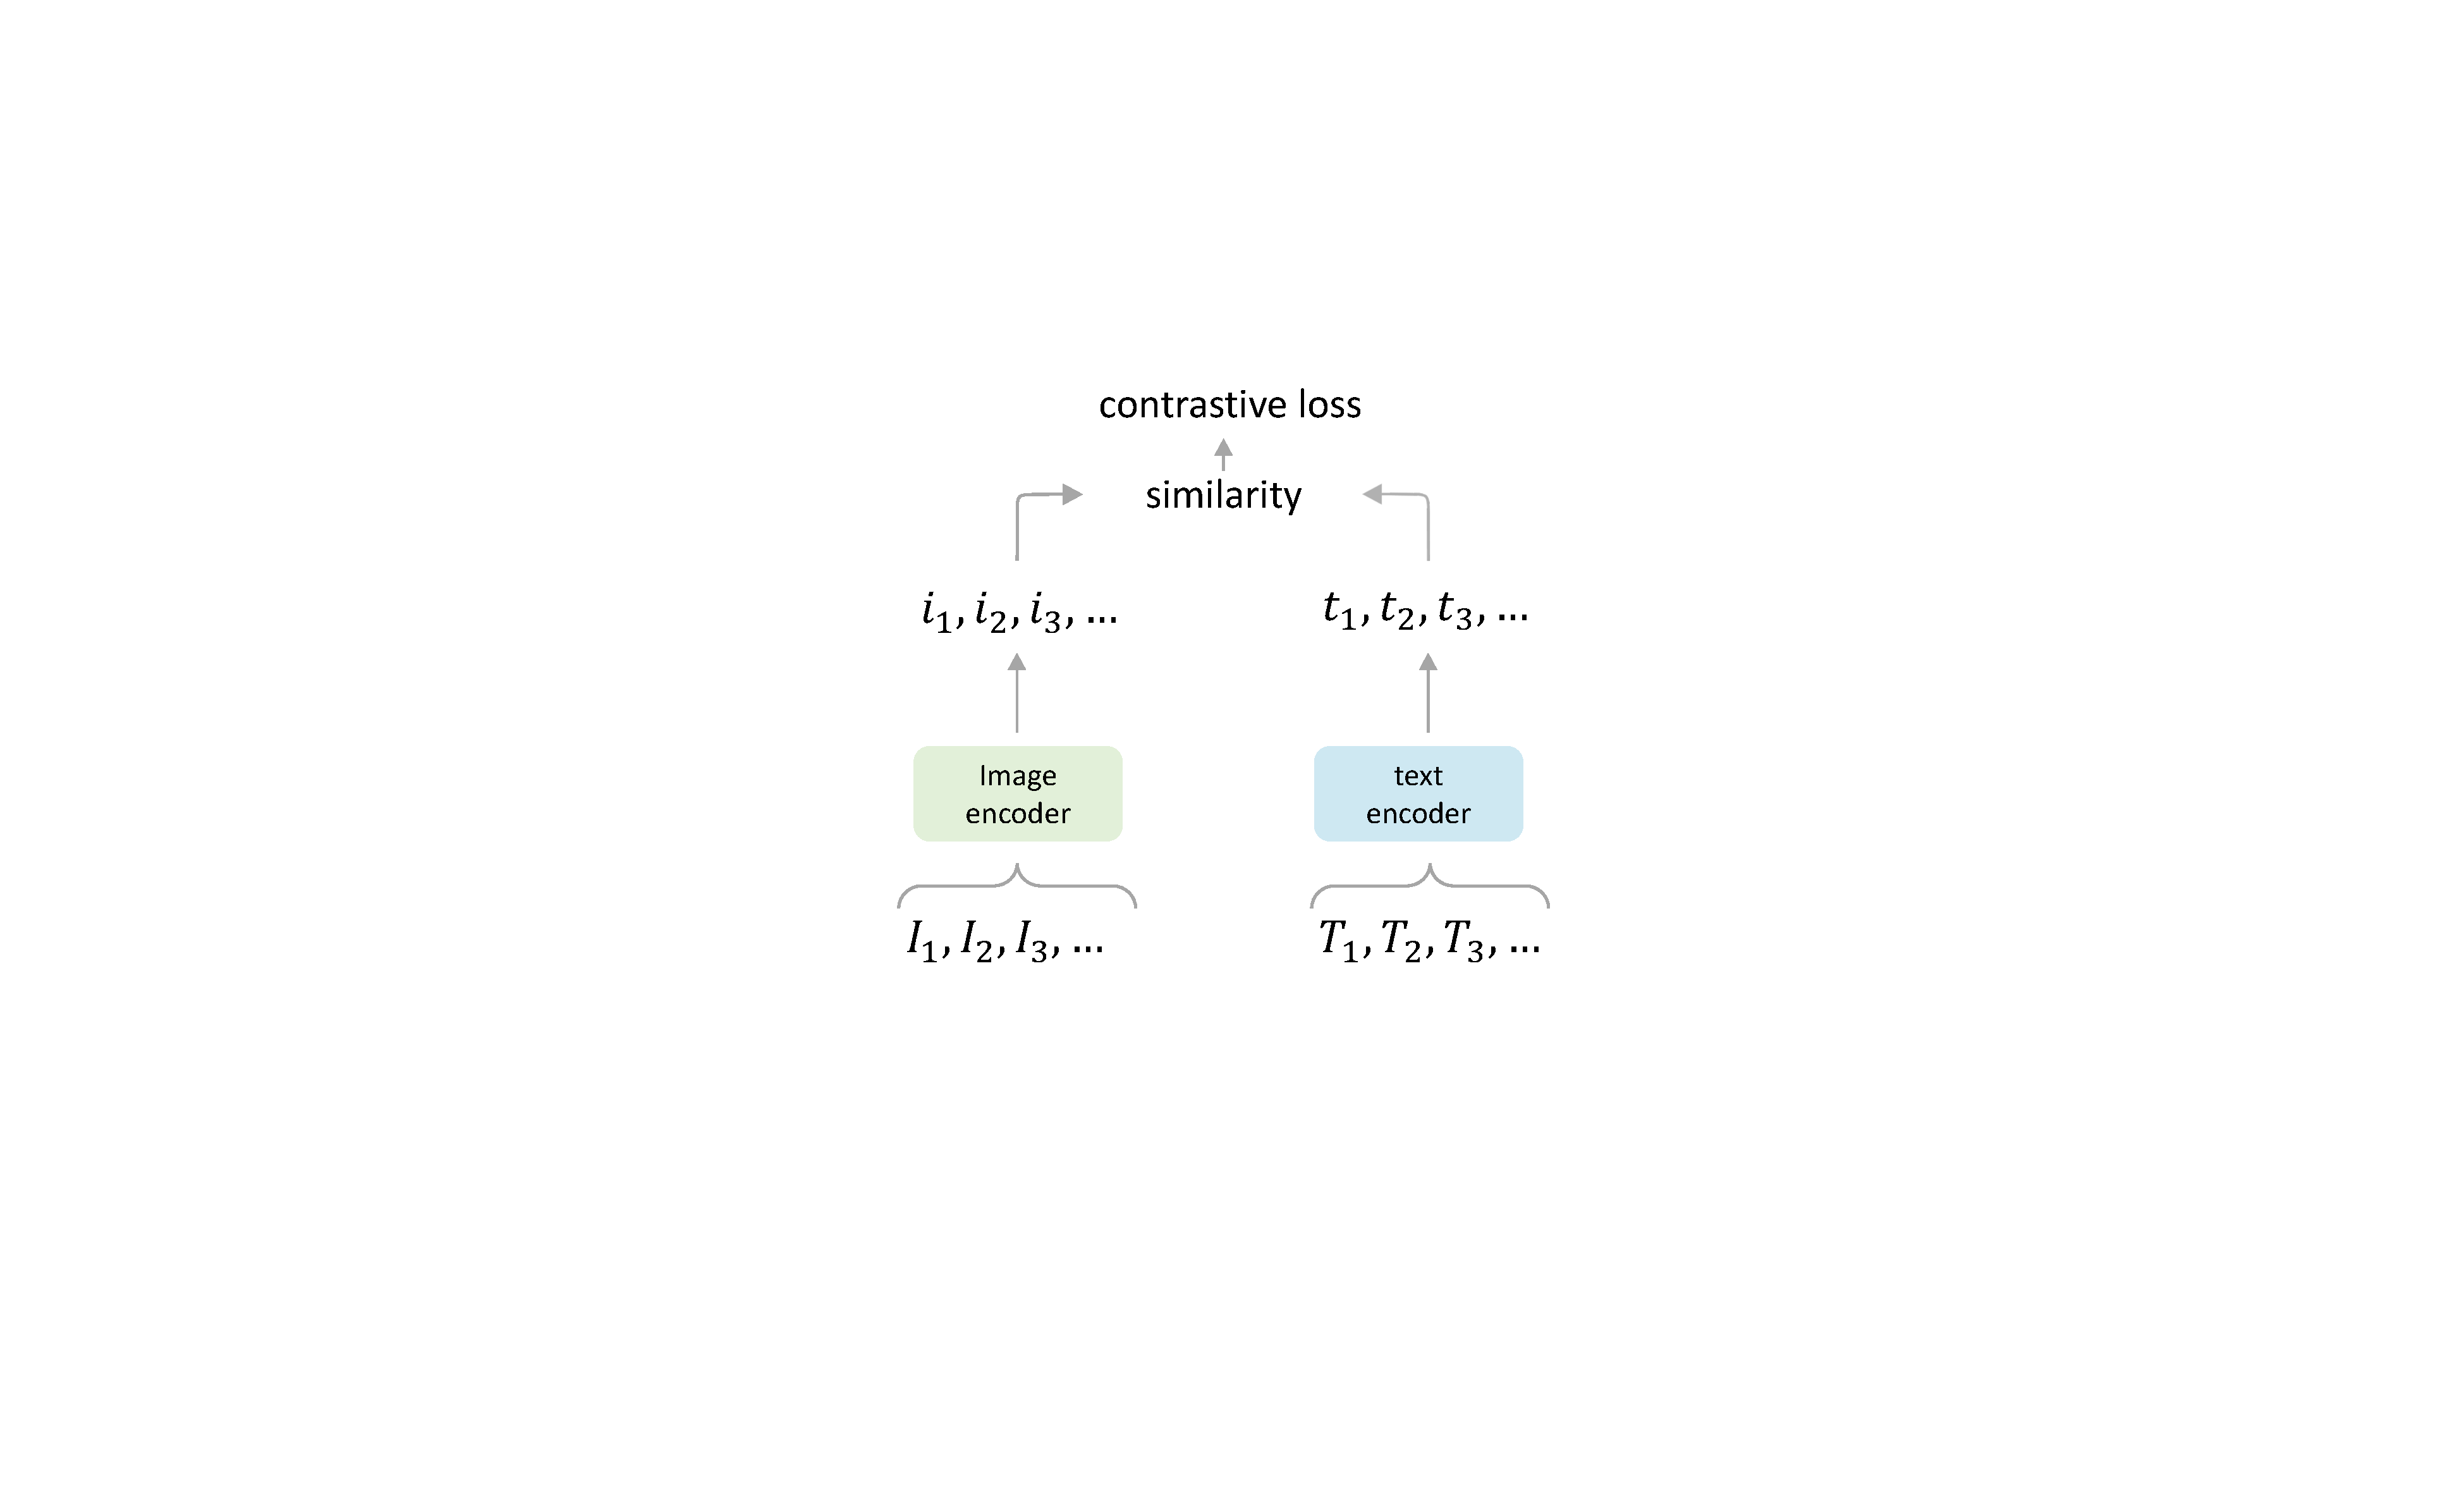
\includegraphics[width=0.5\textwidth]{assets/charts_rw/CLIP}
    \caption[Illustration of CLIP Model Structure]{This figure illustrates the structure of CLIP model. The left stream encodes images, while the right stream encodes text. Both streams are embedded into the same semantic space. Source: \parencite{radford2021learning}}
    \label{fig:clipstructure}
\end{figure}

With these advantages, CLIP has been utilised in several image downstream tasks including few-shot learning \parencite{zhang2022tip}, segmentation \parencite{wang2022cris}, video retrieval \parencite{ma2022x}, object detection \parencite{lin2023gridclip}, and captioning \parencite{mokady2021clipcap}. In addition, CLIP for videos has also been proposed \parencite{xu-etal-2021-videoclip, wang2022internvideo}, achieving state-of-the-art results in several video downstream tasks such as classification, video retrieval, and vision question answering.

This research focuses on the long-tail issue and has demonstrated that the text encoder of pretrained CLIP is an efficient tool to overcome the scarcity problem of tail classes.


\section{Temporal Redundancy}
It is shown that boundaries of objects in frames or any small displacements between neighbouring frames are significant features for action recognition \parencite{10.1007/978-3-030-12939-2_20}. In order to enhance the model in this aspect, optical flow and pretext learning are two research directions. 

\subsection{Optical Flow}
In order to capture subtle boundary changes between frames, integrating optical flow as an independent stream within the model structure has gained popularity for action recognition \parencite{sevilla2019integration, tran2015learning, carreira2017quo}. For instance, the I3D architecture \parencite{carreira2017quo} employs a 3D CNN on both the RGB stream and the optical flow stream, followed by their summation to produce the final prediction, as illustrated in (e) of Figure \ref{fig:structuresi3d}. As Figure \ref{fig:structuresi3d} illustrates, it compares its structure to other four networks, two of which incorporate optical flow as an independent stream for action recognition.

\begin{figure}[ht]
    \centering
    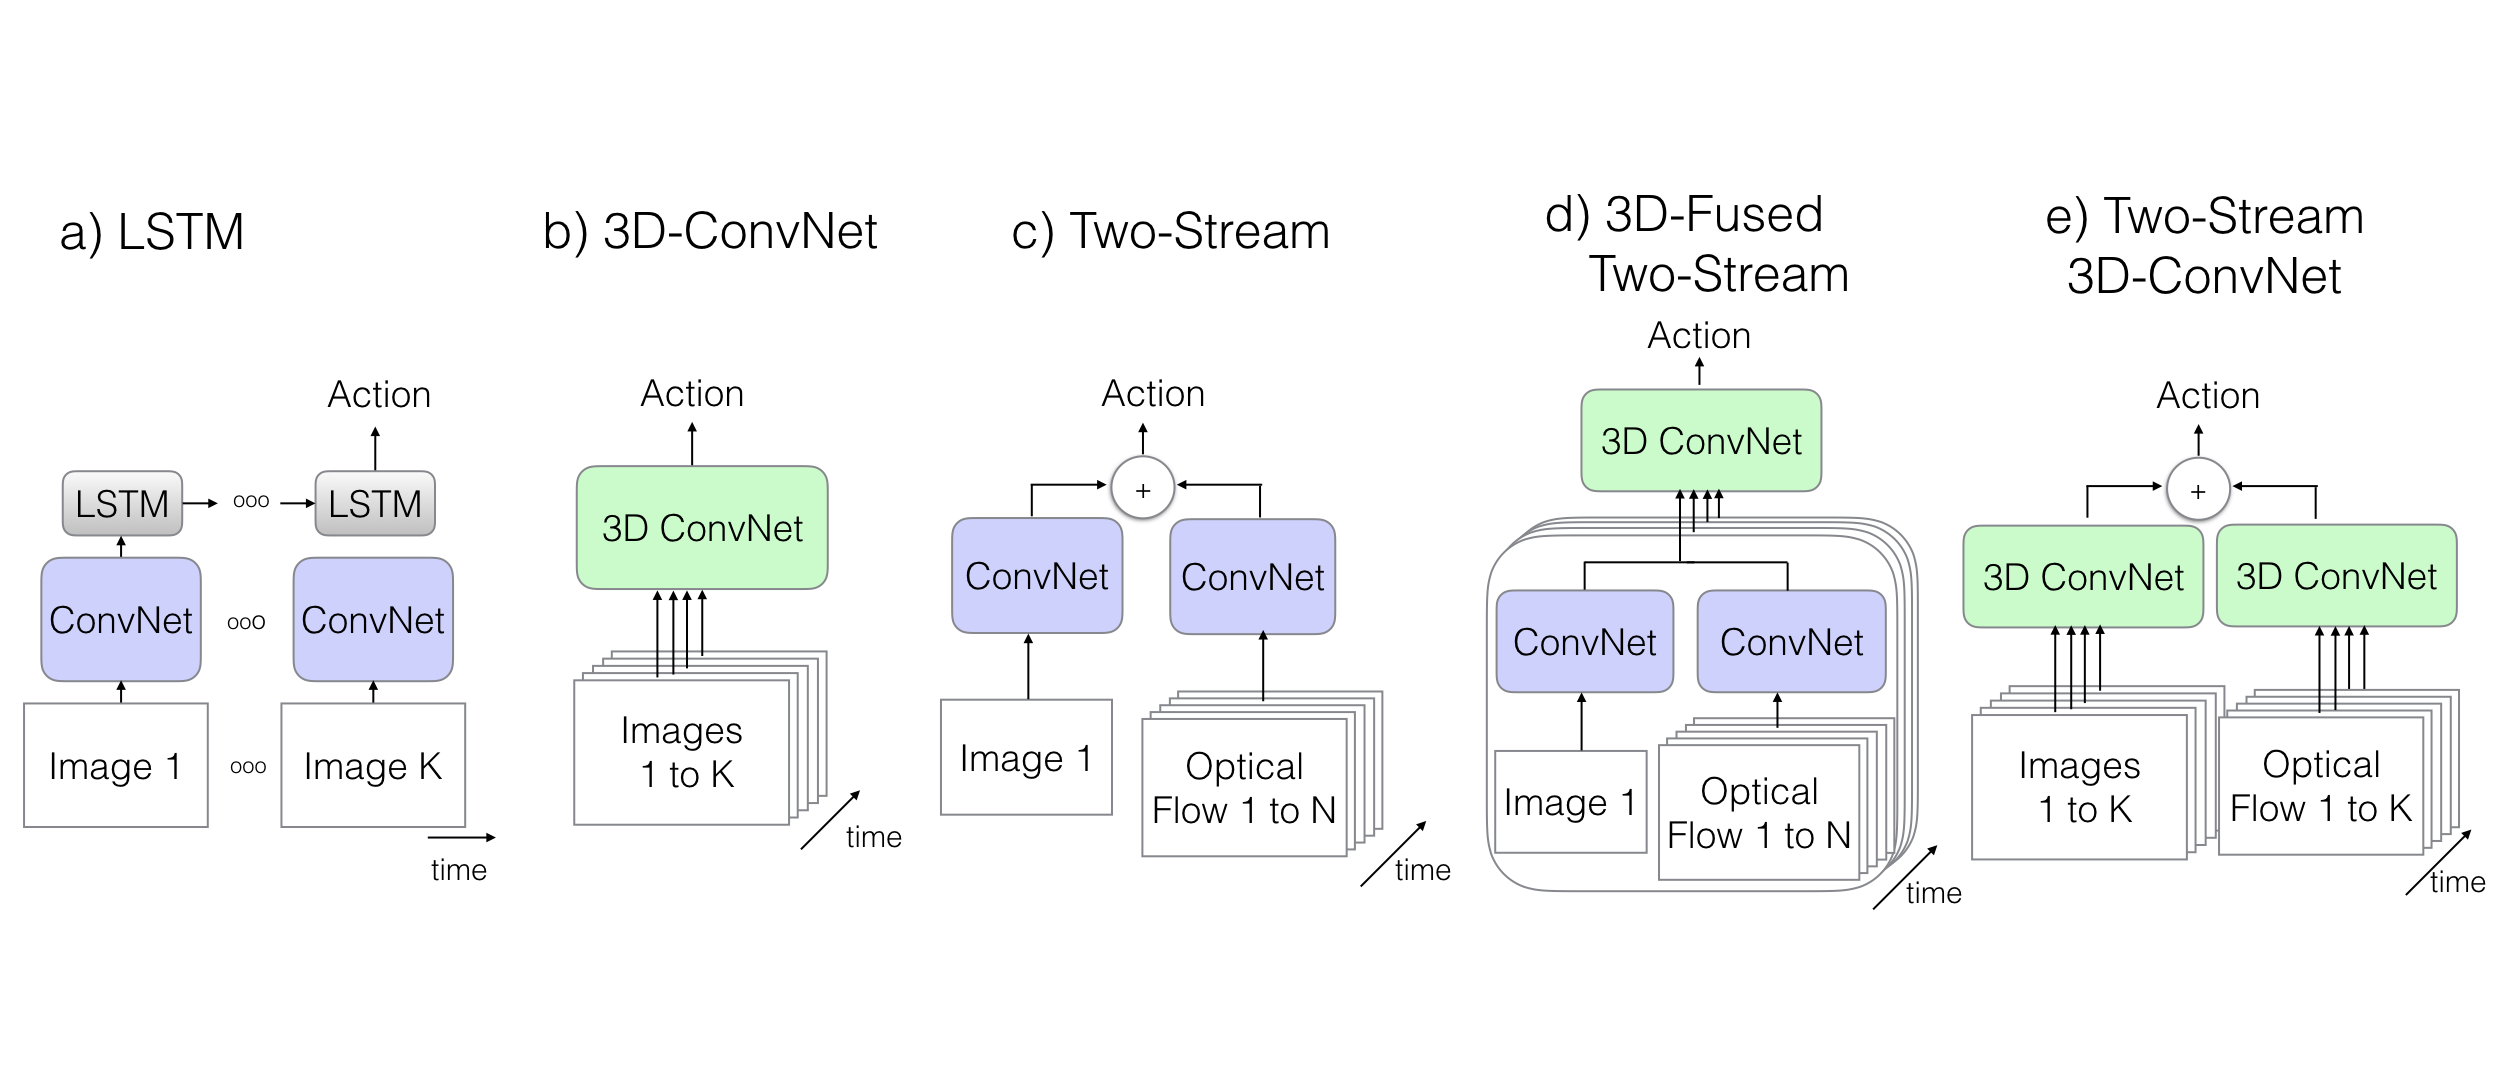
\includegraphics[width=1.0\textwidth]{assets/charts_rw/I3D}
    \caption[Illustration of Structures Discussed in I3D]{This figure illustrates the structures discussed in I3D paper. Subfigure (e) is the structure of I3D. Source: \parencite{carreira2017quo}}
    \label{fig:structuresi3d}
\end{figure}

Some studies have suggested that optical flow may be replaced or improved due to the expensive computing resources used for its calculation. They proposed another network to substitute the pretrained optical flow model with structural improvements that capture motion between frames, an end-to-end classification network that also predicts the optical flow map. However, although they were more advantageous in terms of the number of model parameters and computation speed, they suffered from inferior performance \parencite{Lee_2018_ECCV, 8354283, Piergiovanni_2019_CVPR}.

\subsection{Pretext Learning}
Some more recent studies focus on designing different pretext tasks for the model to learn in a self-supervised way \parencite{wang2022internvideo}.

Through careful design, the pretext learning can empower the model to produce high-quality visual representation in a specific semantic space, which can further be used in downstream tasks such as action recognition, video retrieval, or video captioning \parencite{10.1145/3577925}.

Some studies train models to predict appearance statistics \parencite{Wang_2019_CVPR}, rotation angles \parencite{DBLP:journals/corr/abs-1811-11387}, playback speed \parencite{Yao_2020_CVPR, 10.1007/978-3-030-58520-4_30}, and temporal order \parencite{10.1007/978-3-030-58604-1_26}. Another approach involves the design of contrastive learning models that determine whether two augmented images originate from the same source. Notable examples include MoCo \parencite{finn2017model} and SimCLR \parencite{pmlr-v119-chen20j}. The latter, SimCLR, processes two views augmented from a single image, and its objective is to maximize their similarity in the embedding space. these methodologies have been extended for application in the video domain \parencite{Feichtenhofer_2021_CVPR}.

Inspired by SimCLR, an Action Frame Contrastive Learning Network (AFRICAN) is proposed in this research to force the model to capture the fine-grained difference between frames in a video. In the pretraining stage of AFRICAN, frames in a video are augmented into two different views to do contrastive learning. The target of the contrastive learning model is to identify pairs of frames from the same frame source. This way, the model is able to explore weights that can capture the fine-grained difference between frames. 
